\documentclass[conference]{IEEEtran}
\usepackage[english]{babel}
\usepackage{amsmath}
\usepackage{graphicx}
\usepackage[hypcap=false]{caption}
\usepackage{subcaption}
\graphicspath{ {./images/} }
\usepackage{hyperref}
\hypersetup{
	hidelinks
	}

\title{DAT Midterm Project: Working Title}
\author{Brandon Hosley}
\date{\today}

\begin{document}
	\maketitle
	
\begin{abstract}
	%
	%	content...
	%
\end{abstract}

\section{Introduction}

Shooting sports are a type of sport inextricably linked to technology, 
both in terms of the equipment used by the athletes and tools used in their training.
There is substantial interest in maintaining the cutting edge on both fronts as athletes and teams work to remain on top of their competition.
Access to this type of technology comes with a substantial price, which may be suitable to professional athletes or clubs and individuals of greater means.
Due to the high cost, some highly talented athletes may never get access to high quality equipment or training.

In this paper we propose to develop a two-part open source framework for training that my accomplish the following:

\begin{enumerate}
	\item Recording the Shot Cycle
	\begin{enumerate}
		\item Identify the bull's-eye as a frame of reference.
		\item Identify the point of aim in real-time.
		\item Record the point of aim over the period of an entire shot cycle.
		\item Record actual shot position
	\end{enumerate}
	\item Reporting the Shot Cycle
	\begin{enumerate}
		\item Report the above information in an intuitive manner, that may be interpreted by the athlete and to allow for immediate feedback.
		\item Use the shot position to provide the score and direction.
	\end{enumerate}
\end{enumerate}

With these functions we desire to advance the field of open source options for shooting athletes to improve their craft in a manner functionally similar to the commercial offerings \cite{scatt, noptel} that may otherwise be out of reach.
% ShootOff is a similar laser spot tracker, but only tracks the shot

\section{Related Work}

\subsection{Similar Open-Source Tools}

First we examine work that similarly looks to address the problem of high cost associated with competitive equipment.
At the time of this writing the available open-source options all address the problem of shot scoring.
Traditionally, target scoring is performed using Piezo-electronic sensor to achieve acoustic triangulation \cite{Anderson2018}.
However, some manufacturers have had success with laser triangulation \cite{SUIS}.
In response to the price of this equipment some developers have produced open source projects featuring acoustic scoring \cite{etarg, freetarget}.
Still more researchers have sought to use computer vision to perform the scoring \cite{Rudzinski2012, Stenhager2021}.

Accurate scoring with computer vision and commonly available parts continues to progress rapidly in recent years.
\cite{Ye2011} reliably produced  hit-miss results while \cite{Rudzinski2012} were able to produce competition level accuracy in scoring static targets with the trade-off of extremely controlled reading conditions.
More recently \cite{Stenhager2021} was able to achieve a fairly robust model that could perform in a realistic setting and gave results usable at an amateur level; their system unable to accurately score a round at the necessary resolution.

\subsection{Aim tracing}

\begin{figure}[]
	\centering
	\includegraphics[width=\linewidth]{perfect_shot}
	\caption{SCATT \cite{scatt} feedback.}
	\label{fig:SCATT_Example}
\end{figure}

\begin{figure}[]
	\centering
	\includegraphics[width=0.6\linewidth]{mantisx_output}
	\caption{MantisX \cite{mantisx} output.}
	\label{fig:MantisX_Example}
\end{figure}

Shot scoring is only one aspect of training, and dry-fire training is often 
considered to be the most important for developing a training regimen with effective results
\cite{Potter2017}.
This importance is reflected in shot trainers that sometimes cost as much as the top of the line equipment itself
\cite{scatt, noptel}.

Both the Noptel and SCATT systems utilize computer vision for their tracking.
They utilize the relative positioning of the bullseye within the camera's field of view to determine the position of the aim.
Actual point of aim is calibrated by having the weapon fire and recording where in the frame the resulting hole is observed.
The cameras use an uncommon lens configuration for the optical zoom which produce effective results for their intended purpose, but are not likely useful in other applications.
Conversely, cameras of this type are not easily sourced from other applications.

The Mantis X \cite{mantisx} product utilizes an inertial measurement unit that has been ruggedized against small arm recoil. 
This product does not utilize a camera and is not able to produce a prediction of a point of aim.
Instead the output is a trace of relative position and will correlate the relative positions to the position when the weapon is fired.
In this way it can still produce data valuable to the shot cycle without actually being able to score.
The advantage is that it may eschew any visual obstacles or shortcomings.
This product also utilizes very niche components that are not ideal for open source.

The commercial trainers share a set of common features and outputs,
in addition to collecting the point of aim these software break up the trace into several parts:
\begin{enumerate}
	\item Entry onto target and sighting
	\item Triggering (approximated as 1 second before impact)
	\item Shot (0.3 seconds before impact)  and Impact
	\item Follow-through and leaving the target
\end{enumerate}
For ease of interpretation each of these stages are delineated by color; the schema presented by SCATT can be seen in figures 
\ref{fig:SCATT_Example} and
\ref{fig:MantisX_Example}.


\section{Dataset}

All of the data sets that we encountered during the preliminary research for this project utilized proprietary storage methods.
While one site was able to use a framework that retrieved the actual shot results from SCATT traces \cite{scatt-db}, that particular framework was not able to retrieve the trace data itself.

To address this we use an easier to ingest data storage method, trading potential gains in efficiency when using binaries for ease of access.


\section{Methods}

The hardware used for this experiment was 
a Microsoft Lifecam HD-5000,
a Steyr evo 10 E,
and a red laser pointer of unknown origin.
All recording, processing, and analysis was performed on 
a 2020 Apple M1 Macbook Pro.

Video capture and processing was performed using the 
OpenCV \cite{itseez2015opencv} framework as a base.
The bullseye area is used as a fiducial for recording and 
the necessary data is determined by applying a series of OpenCV functions.

\begin{figure}[]
	\centering
	\includegraphics[width=0.75\linewidth]{example-image}
	\caption{Recording Algorithm.}
	\label{fig:capture_algorithm}
\end{figure}

The first step is to import the frame as a hue, saturation, value image.
Then a mask is applied to filter for only the near-black area.
A contour is applied to the outer edge of the mask.
The moments of the outer contour are calculated.
The first order moment of each dimension is divided by the zeroth moment to determine the center coordinate for the corresponding dimension.
$M_{10}$ and $M_{01}$ each divided by $M_{10}$ using eq. \eqref{Moments}.
Finally, a minimum enclosing circle is applied around the contour and used to provide an approximate radius.

\begin{equation}\label{Moments}
	\text{Moments} = M_{ij} = \sum_{x} \sum_{y} x^i y^j I(x,y)
\end{equation}

A Hough Circle Transform solution \cite{Hough1964} was considered for producing both of these data.
However, the results were extremely unstable when applied to the conditions used for this experiment and the video capture itself.
Additionally, while this method may have been more accurate for determining the true center of the target, it would not work well for an ellipsoid reference.
This problem is discussed further in the conclusion of this paper.

The moment of the bullseye will be referenced as the origin for plotting the other points. 
The radius will be used to normalize the reported coordinates of the marker so they are recorded in absolute terms.
This will allow the results to be consistent among various recording distances and various sizes of camera views.
However, it does require that the radius of the bullseye can be input into the script.
For common, standardized targets this information is easily accessible
\cite{issfRules} and may added to a more refined version of this program.
The measurements for this are based on the average of 100 iterations to improve the stability of the readings.

Predicting an origin for the target and basing the trace off that origin produced better results than attempting to identify a new origin periodically during the video capture.
We believe this to the result of adding an additional variable in which anomalies can amplify anomalies resulting from the laser position prediction. 
Additionally, the color and brightness of the laser changed the shape of the target center and had the effect of biasing the predicted origin away from the true center in the direction opposite of the laser.
Finally, attempting to predict the origin with a great enough frequency to overcome anomalous readings the performance of the script was reduced below a usable level.

The second, and recurring part of the script is the capturing the position of the laser which followed a similar image processing algorithm as the fiducial identification portion.
This stage ignores the outer boundaries and size of the laser and attempts to find the center.

The surface of standard competition targets causes the laser to reflect diffusely.
The diffusion caused the marker to appear as a highly irregular ellipsoid,
however, when the angle of incident is low the moment is still an effective measure of center for the marker.
This was not a problem with the dark area of the bulls-eye as it was far less reflective.

To overcome the irregularity, and improve the stability of the readings, the script will attempt 3 readings, and average the results.
This has the added benefit of reducing the record speed and preventing the script from needlessly recording data without meaningful differences from the previous point.

\begin{figure}[]
	\centering
	\includegraphics[width=\linewidth]{screen_cap3}
	\caption{Capture of the OpenCV frame.}
	\label{fig:screen_cap}
\end{figure}

The result of these functions can be seen in figure \ref{fig:screen_cap}.
In this example a blue circle is drawn around the fiducial,
a green dot placed at it center represents the predicted origin, and
a red dot is placed at the center of the detected marker.

The position of the laser, and the estimated point of aim, is recorded in millimeters as a pair of coordinates on a Cartesian plain. 
These coordinates and the time are fed into an array which is exported at the conclusion of the trace recording.

The timer and the recording start at the first detection of a laser in the field of view.
The trace concludes after a certain period of time passes without any new position recordings.

For the purposes of this implementation the actual database is eschewed in favor of simpler comma separated values files.

\begin{figure}[]
	\centering
	\includegraphics[width=0.75\linewidth]{example-image}
	\caption{Database.}
	\label{fig:database}
\end{figure}


\section{Analysis}

The output of the tracking algorithm is easily digestible with common data visualization techniques.
Several proposals for analysis and the visualization of this information are presented in this section and will be shown and training value discussed in the next section.

The scalar distance over time can help the user evaluate several aspects of their shot cycle without the distractions of actual placement on the recreated target,
but is not a visualization provided by other implementations.
By plotting directly against the time variable certain parts of the shot cycle
\cite{Zeljko2020}
can be more closely examined.
This is accomplished by converting the Cartesian coordinates to Polar and plotting the $\rho$ variable against time.
In this format specific times of the cycle may be examined.
Of particular note is the entry onto target and directness of the approach to center.
This slope should take a similar shape to the slope of the point of aim leaving the target, any deviations will suggest an uneven or erratic entry movement.
The movement at the time of triggering and the first part of the follow-through may also be more easily examined in this format.

While the scalar mode may assist the user in understanding events in the shot cycle that occur at specific times, to improve positional feedback we provide a heatmap.
The heatmap is produced using a Gaussian filter which will help normalize the distribution of positions.
This visual is intended to show the user where the point of aim spends the most time and may highlight directional bias that might not otherwise be obvious with the other trace playback methods.

\section{Results}

\begin{figure}[]
	\centering
	\includegraphics[width=\linewidth]{trace}
	\caption{Trace replay.}
	\label{fig:trace}
\end{figure}

In figure \ref{fig:trace} the replay of a shot may be seen.
It is presented in a manner similar to figure \ref{fig:SCATT_Example}, 
though with inferior technique.
The movement is wider and spends less time at the center of the target compared to the nearly perfect shot of  \ref{fig:SCATT_Example}
One way this can be shown is the scalar over time in figure \ref{fig:dfc}.

\begin{figure}[]
	\centering
	\includegraphics[width=\linewidth]{distance_from_center}
	\caption{Scalar distance and time}
	\label{fig:dfc}
\end{figure}

Next we examine the heatmap visual presented in figure \ref{fig:heatmap}.
This example highlights a bias toward the lower left quadrant that is not obvious when compared to figure \ref{fig:trace}.


\begin{figure}[]
	\centering
	\includegraphics[width=\linewidth]{heatmap}
	\caption{Trace heatmap.}
	\label{fig:heatmap}
\end{figure}









\section{Conclusion}

As a proof-of-concept this project has successfully shown that it is possible to record an athlete's point of aim with cheap and widely available materials.
However, the implementation produced for this project is far from robust and still requires strong caveats on its usage.
The shortcomings and difficulties will be listed in this section, 
and ideas for improvement and future experiments will be discuss in the next section.

The diffuse reflection mentioned in the method section did cause some problems, especially when the marker was crossing from the light areas of the outer target to the dark area of the bullseye which experienced a lot less diffusion.
This distortion had a tendency to bias the readings of the marker toward the outer edge of the bullseye area.
Additionally, if the user did not maintain a shallow angle of incidence with the laser the diffusion would bias the readings in the opposite direction from the user.

Because this computer vision task utilizes light reflecting off a flat surface the algorithm cannot use edges and must instead rely on color or changes in image.
The reliance on color makes this implementation sensitive to changes in lighting condition and the webcam's color gamut.

\subsection{Areas for Improvement}

The method used to evaluate the bullseye reference frame does not compensate for the viewing angle. Instead of using a circular-bound it will need to use an ellipsoid and additional transformations will need to be applied to more accurately place the trace on the target.

Unlike the software that inspired this project there is no user friendly way to calibrate the laser emitter to the proper placement relative to the sights.
The most common method used is to require the user to place at least one live shot onto the target, though multiple are often recommended.
The program will then identify the actual placement of the shot and correlate that position to the frame provided by the camera.
This can be seen in figure \ref{fig:scatt_calibration} where three shot positions are averaged to produce the point of aim relative to the optical sensor's field of view.

\begin{figure}[]
	\centering
	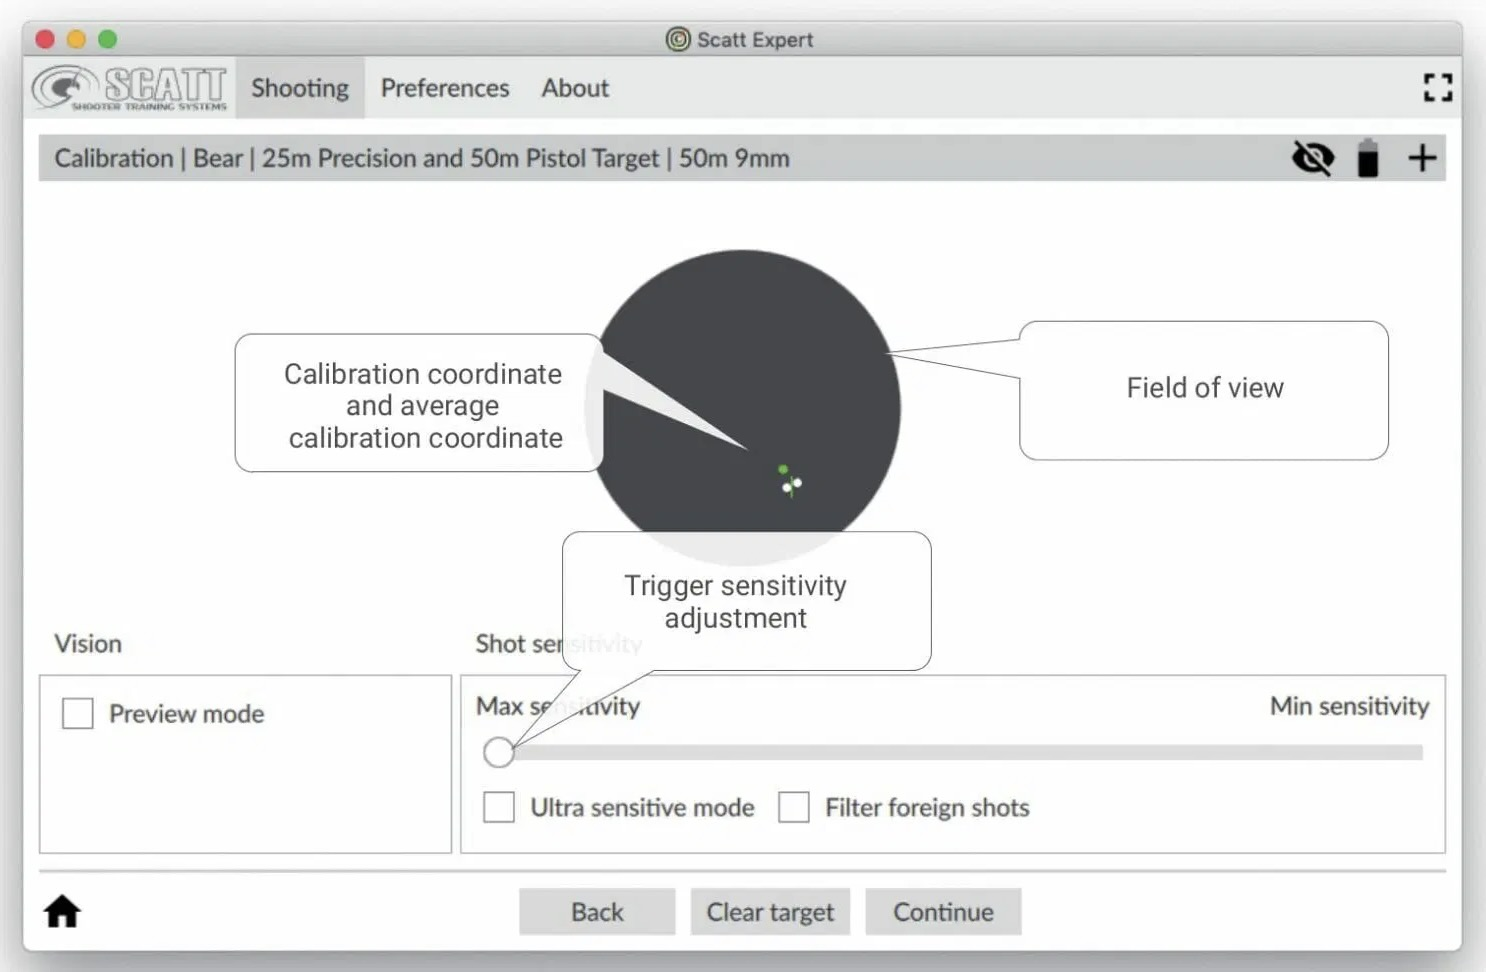
\includegraphics[width=\linewidth]{scatt_calibration}
	\caption{Scatt \cite{scatt} calibration menu.}
	\label{fig:scatt_calibration}
\end{figure}


\subsection{Future Work}

Future work on this project will include attempts to have the algorithm identify the marker in ways that are less sensitive to lighting.
One such method may be comparing changes between frames,
however, this will potentially need to compensate for wind disturbance.

Another line of effort will be to source commonly available parts from other applications, specifically, continued use of a webcam and the addition of a small telescopic lens, the type marketed for increasing the focal distance of a cell phone camera.
With these parts we may be able to replicate the method used in the commercial offerings listed earlier.



% 		Expand on open sourced technologies
%			Polycarbonate impact surface and Piezo-electronic vibration sensing
%			Screen Behind for target variation, immediate shot recording and track playback, even with dry-fire training
%		Another Commercial option: https://www.traceshooting.com/?lang=en
%	Helpful for script generation: https://techvidvan.com/tutorials/create-air-canvas-using-opencv-python/
%\clearpage
\bibliographystyle{IEEEtran}
\bibliography{\jobname}
\end{document}